\documentclass[11pt]{amsart}
\usepackage{amsmath}
\usepackage{amssymb}
\usepackage{xcolor}
\usepackage{tikz}

\begin{document}

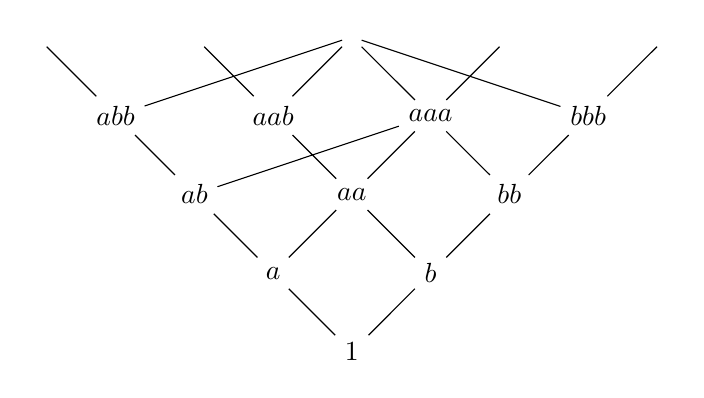
\begin{tikzpicture}
\node (A) at (0,0) {$1$};
\node (B) at (-1,1) {$a$};
\node (C) at (1,1) {$b$};
\node (D) at (-2,2) {$ab$};
\node (E) at (0,2) {$aa$};
\node (F) at (2,2) {$bb$};
\node (G) at (-3,3) {$abb$};
\node (H) at (-1,3) {$aab$};
\node (I) at (1,3) {$aaa$};
\node (J) at (3,3) {$bbb$};
\node (K) at (-4,4) { };
\node (L) at (-2,4) { };
\node (M) at (0,4) { };
\node (N) at (2,4) { };
\node (O) at (4,4) { };
\draw (B) -- (A) -- (C);
\draw (D) -- (B) -- (E) -- (C) -- (F);
\draw (G) -- (D) -- (I) -- (E) -- (H) -- (E) -- (I) -- (F) -- (J);
\draw (G) -- (M) -- (H) -- (M) -- (I) -- (M) -- (J);
\draw (G) -- (K);
\draw (H) -- (L);
\draw (I) -- (N);
\draw (J) -- (O);

\end{tikzpicture}

\end{document}